\section{GUI}

\subsection{Indledning}
Da et af de sekundære mål var at afsende billeder, ville det være fordelagtigt at bruge en grafisk brugerflade istedet for konsollen, så istedet for at åbne et billede som billedefil, var meningen at få billedet frem i selve chat vinduet.

Den grafiske brugerflade blev udviklet ved hjælp af QT, et program som er bygget op om C++ syntax, QT er brugervenligt og let at lære at skrive, hvis C++ allerede er et kendt programmeringssprog.\\
\subsection{Funktionalitet}

I den grafiske brugerflade er der 3 elementer.
\begin{itemize}
	\item Chat boks, hvori selve chatten foregår, her kommer der til at stå hvad der modtages, samt hvilket input der gives.
	\item Send knap denne afsender den tekst som er skrevet i chat linjen.
	\item Chat linje, dette er hvor input fra brugeren kommer til at stå, når der skrives noget, og trykkes enter / send, bliver beskeden afsendt.
\end{itemize}

Når der skrives noget i chat linjen, og der trykkes på enter, så kaldes en funktion fra applikationslaget som hedder send, som tager en streng som parameter, denne streng er så indput fra chat linjen.

\subsection{Delkonklussion}
Den grafiske brugerflade blev valgt til at være et helt standard chatvindue som set på figur \ref{fig:GUI}.
Brugerfladen blev ikke implementeret da der var problemer med at holde en sideløbende tråd kørende samtidig med brugerfladen, dette blev opdaget for sent og der var ikke tid til at fejlfinde, derfor blev alternativet konsollen, samtidig var målet med at afsende billeder ikke blevet nået så den grafiske brugerflade var ikke så nødvendig.




\begin{figure}[h]
\centering
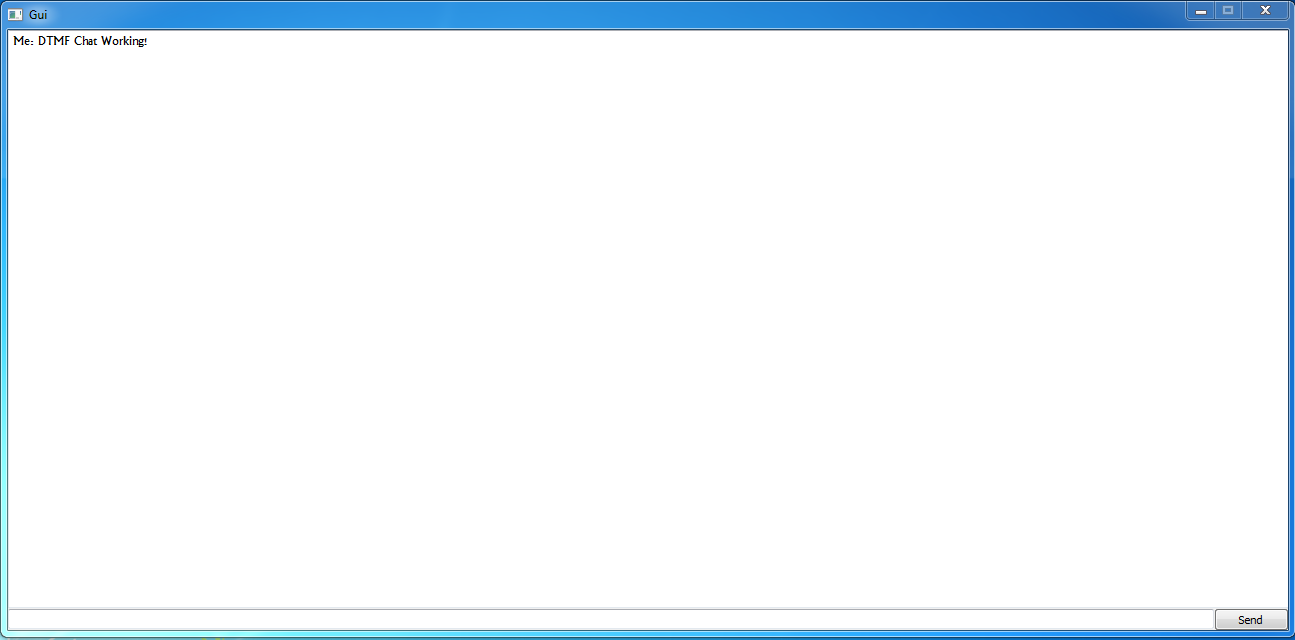
\includegraphics[scale=0.5]{Billeder/GUI.PNG}
\caption{Den Grafiske Brugerflade}
\label{fig:GUI}
\end{figure}